\chapter[Uncertain time series u-shapelet discovery]{Frobenius correlation based u-shapelets discovery for time series clustering}

\begin{abstract}
An u-shapelet is a sub-sequence of a time series used for clustering a time series dataset. The purpose of this paper is to discover u-shapelets on uncertain time series. To achieve this goal, we propose a dissimilarity score called FOTS whose computation is based on the eigenvector decomposition and the comparison of the autocorrelation matrices of the time series. This score is robust to the presence of uncertainty; it is not very sensitive to transient changes; it allows capturing complex relationships between time series such as oscillations and trends, and it is also well adapted to the comparison of short time series. The FOTS score is  used with the Scalable Unsupervised Shapelet Discovery algorithm for the clustering of 17 datasets, and it has shown a substantial improvement in the quality of the clustering with respect to the Rand Index. This work defines a novel framework for the clustering of uncertain time series.
\end{abstract}

\section{Introduction}
Uncertainty in time series comes from several sources.  For instance, to protect privacy, privacy-preserving transformation \cite{papadimitriou2007time, aggarwal2008unifying} deliberately introduce uncertainty to the confidential data before further processing. In a sensor
network, sensor readings are imprecise because of the presence of noise generated either by the equipment
itself or other external influences \cite{cheng2003evaluating}. Ignoring the uncertainty of the data
can lead to rough or inaccurate conclusions, hence the need to implement uncertain data management techniques. 


Several recent studies have focused on the processing of uncertainty in data mining. Two main approaches allow to take uncertainty into account in data mining tasks: either it is taken into account during the comparison by using appropriate distance functions \cite{Rizvandi2013, Hwang2014, Rehfeld2014, Orang2014, Wang2015, Orang2017}, or its impact is reduced by transformations performed on the data
\cite{Orang2015}.This latter strategy is used natively by the u-shapelet algorithm.

\subsection{U-shapelets algorithm for clustering Uncertain Time Series }

U-shapelets clustering is a framework introduced by\cite{zakaria2012clustering} who suggested clustering time series from the local properties of their sub-sequences rather than
using their global features of the time series \cite{zhang2016unsupervised}. In that aim, u-shapelets clustering first seeks a set of sub-sequences characteristic of the different categories of time series and classifies a time series according to the presence or absence of these typical sub-sequences in it. 

Clustering time series with u-shapelets has several advantages. Firstly, u-shapelets clustering is defined for datasets in which  time series have different lengths, which is not the case for most techniques described in the literature. Indeed, in many cases, the equal length assumption is implied,
and the trimming to equal length is done by exploiting expensive human skill \cite{ulanova2015scalable}.  Secondly, u-shapelets clustering is much more expressive regarding representational power. Indeed, it allows clustering only time series that can be
clustered and do not cluster those that do not belong to any cluster.

Furthermore, it is very appropriate to use u-shapelets clustering with uncertain time series because it can ignore irrelevant data and thus, reduce the adverse effects of the presence of uncertainties in the time series. Despite this advantage, it is highly desirable to take into account the adverse impact of uncertainty during u-shapelet discovery.

\subsection{Uncertainty and u-shapelets discovery issue}
Traditional measurement of similarity like Euclidean distance (ED) or Dynamic Time  Warping (DTW) do not always work well for uncertain time series data. Indeed,   they aggregate the uncertainty of each data point of the time series being compared and thus amplify the negative impact of uncertainty. However, ED plays a   fundamental role in u-shapelet discovery because it is used to compute the gap, i.e. the distance between the two groups formed by a u-shapelet candidate. The discovery of u-shapelet on uncertain time series could thus lead to the selection of a wrong u-shapelet candidate or to assign a time series to the wrong cluster.
 
 
 In this study, our goal is to cluster uncertain time series with u-shapelets algorithm. Our work leverages the observation that the use of a dissimilarity function robust to uncertainty could improve the quality of the u-shapelets discovered and thus improve the clustering quality of uncertain time series.

\subsection{Summary of contributions}

\begin{itemize}
  \item We review state of the art on similarity functions for uncertain time
  series and evaluate them for the comparison of small, uncertain time series.  
  \item We introduce the Frobenius cOrrelation for uncertain Time series uShapelet
  discovery (FOTS), a  new dissimilarity score based on local correlation, which
  has interesting properties useful for comparison of small, uncertain  time
  series and that makes no assumption on the probability distribution of
  uncertainty in data.
\item We put the source code at the disposal of the scientific community to
allow extension of our work\cite{expe}.
\end{itemize}
\section[Background]{Definitions and Background}

\subsection{Related work}

An Uncertain Time Series (UTS) $X=<X_1, \ldots, X_n>$  is a sequence of random
variables where $X_i$  is the random variable modeling the unknown real value
number at timestamp $i$. There are two main ways to model uncertain time series:
multiset-based model and PDF-based model.   

\paragraph{}In \textbf{Multiset-based model}, each element $X_i (1 \leq i \leq n)$ of an UTS $X = <X_1, \ldots,  X_n>$ is represented as a set $\{X_{i,1}, \ldots, X_{i,N_i}\}$ of observed values (Fig. \ref{multiset}) and $N_i$
  denotes the number of observed values at timestamp $i$.
  
 \begin{figure}
  \centering
   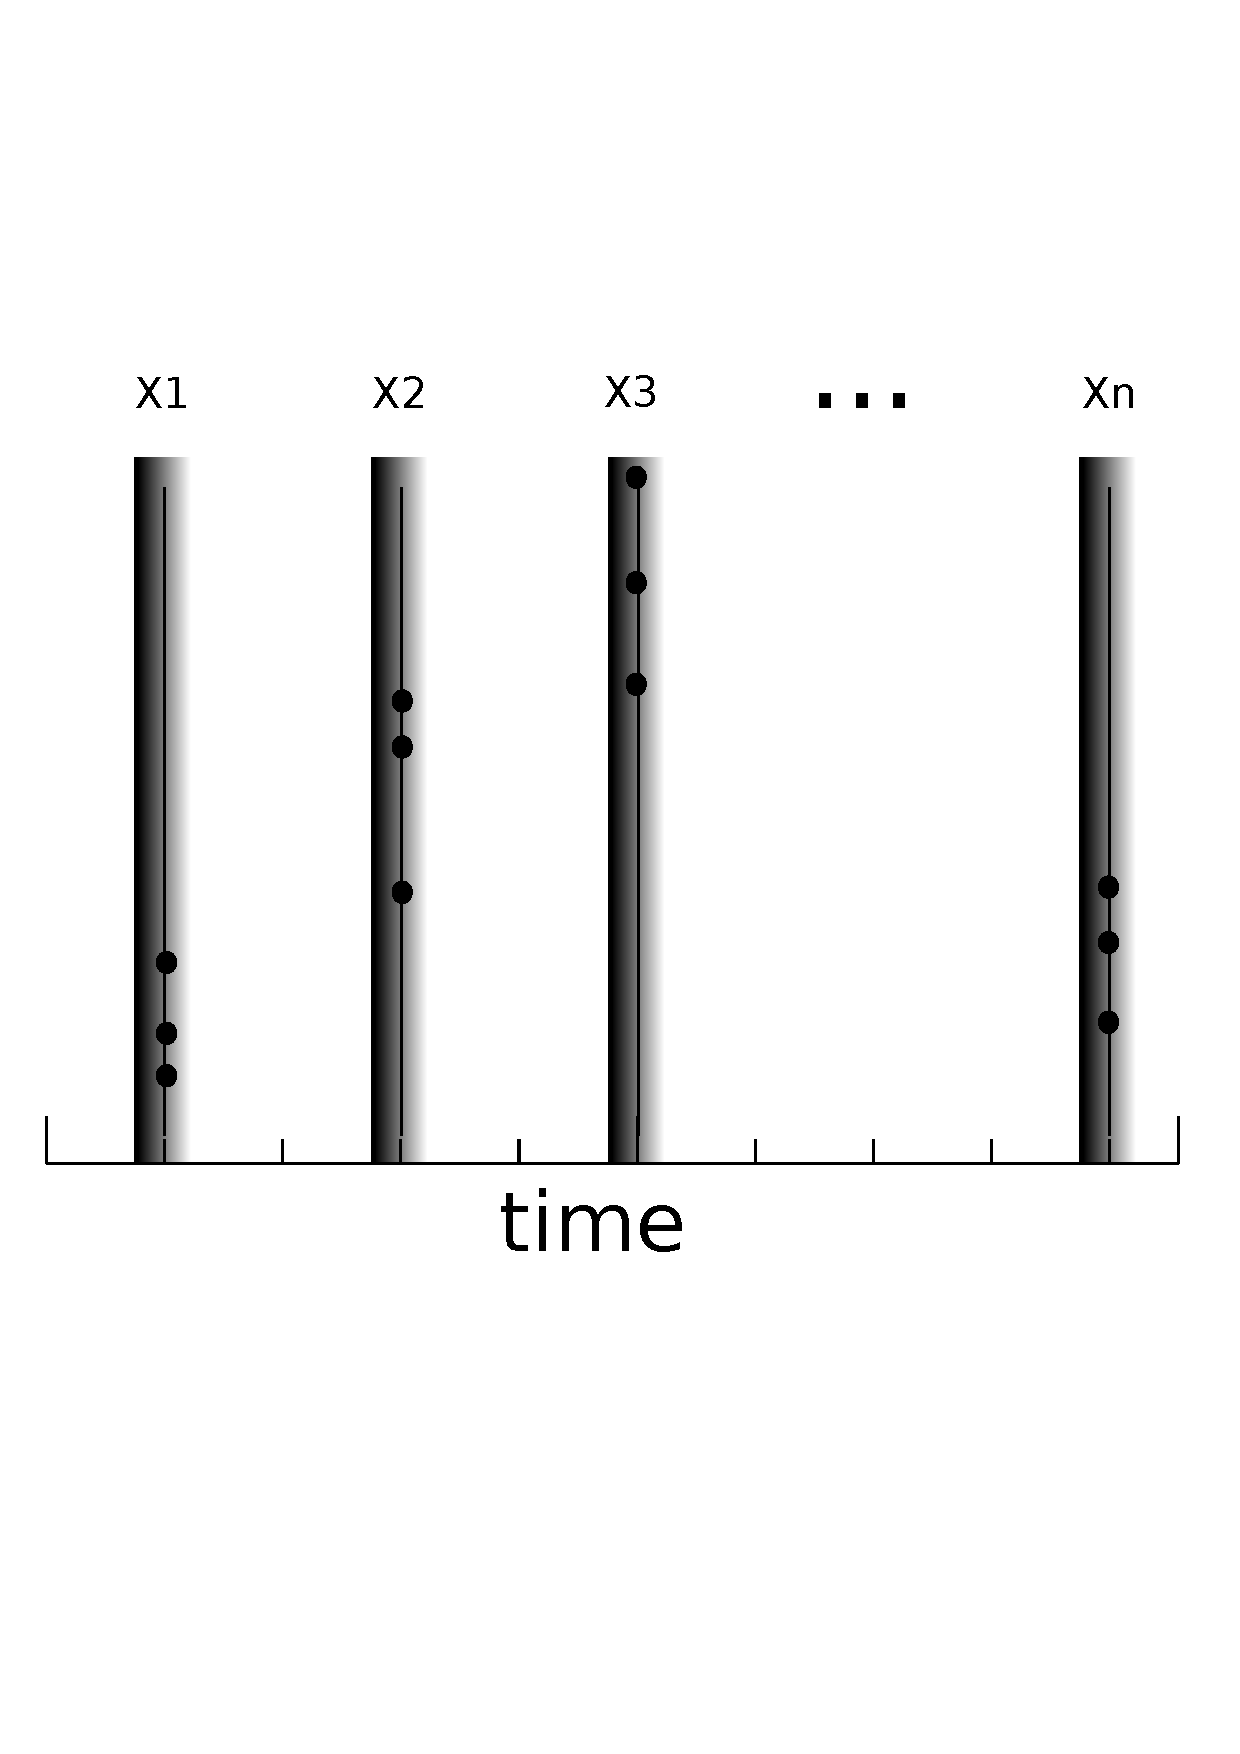
\includegraphics[scale=0.4]{images/multiset2}
    \caption{Multiset-based model of uncertain time series}
  \label{multiset}
  \end{figure}

\paragraph{} In \textbf{PDF-based model}, each element $X_i, (1\leq i \leq n)$ of UTS $X = <X_1, \ldots, X_n>$ is   represented as a random variable $X_i=x_i + X_{e_i}$, where $x_i$ is the exact value that is   unknown and $X_{e_i}$ is a random variable representing the error (Fig. \ref{pdf}). It is this model that we  consider this work.
  
  \begin{figure}
  \centering
   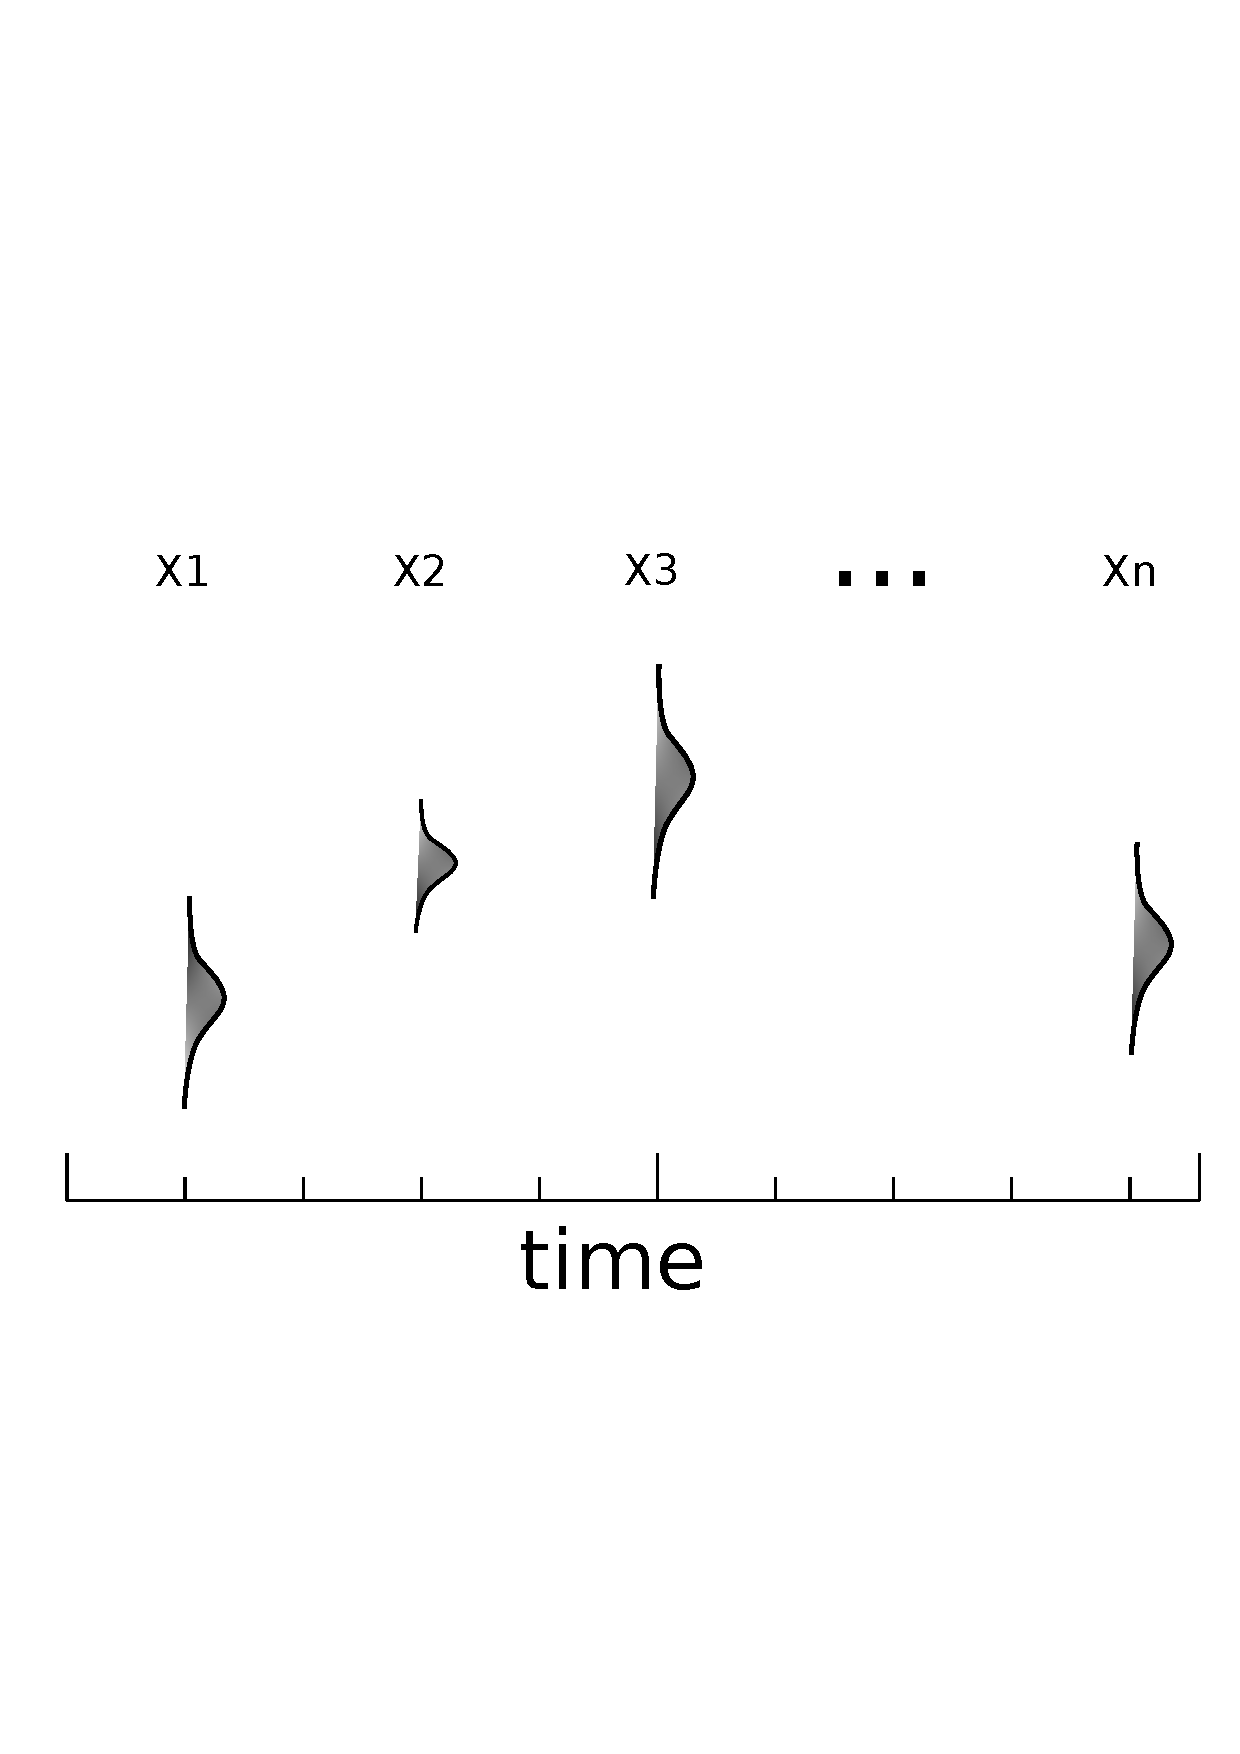
\includegraphics[scale=0.4]{images/pdf2}
  \caption{PDF-based model of uncertain time series}
  \label{pdf}
  \end{figure}
  


Several similarity measures have been proposed for uncertain time series. They are grouped into two main categories: Traditional similarity measures and uncertain similarity measures.

\begin{itemize}
  \item Traditional similarity measures such as Euclidean distance are those conventionally used with time series. They use a single uncertain value at each timestamp as an approximation of
  the unknown real value.
  \item Uncertain similarity measures use additional statistical information that quantifies the uncertainty associated with each approximation of the real value : this is the case of
  DUST, PROUD, MUNICH\cite{dallachiesa}. \cite{Orang2015} demonstrates that the performances of Uncertain similarity measures associated with pre-processing of data are higher than those of traditional similarity measurements.
\end{itemize}


\subsection{Review of u-shapelets}

\begin{definition}
Two datasets  $D_A$ and $D_B$ are said to be \textbf{r-balanced} if only if
$\frac{1}{r}<\frac{|D_{A}|}{|D_{B}|}<(1-\frac{1}{r}),\,r>1$
\end{definition}


\begin{definition}
An \textbf{Unsupervised-Shapelet} is any sub-sequence that has a length shorter than or equal to the length of the shortest time series in the dataset, and that allows dividing the dataset into two
\textbf{r-balanced} groups $D_A$ and $D_B$; where $D_A$ is the group of time series that contains a pattern \textbf{similar} to the shapelet and $D_B$ is the group of
time series that does not contain the shapelet.
\end{definition}

The similarity between a time series and a shapelet is evaluated using a distance function.


\begin{definition}
The sub-sequence distance \textbf{sdist(S, T)} between
a time series T and a sub-sequence S is the minimum of the
distances between the sub-sequence S and all possible
sub-sequences of T of length equal to the length of S.
\end{definition}
This definition opens the question of which distance measure to use for $sdist$.
In general, the ubiquitous Euclidean distance (ED) is used, but it is not
appropriate for uncertain time series \cite{Orang2014}. In the following section, we introduce a
dissimilarity function that is more adapted to  uncertainty.   


Computing the $sdist$ between a u-shapelet candidate
and all time series in a dataset creates an orderline:


\begin{definition}
An orderline is a vector of sub-sequence
distances sdist(S, Ti) between a u-shapelet and all time series Ti in the dataset.
\end{definition}

The computation of the orderline is time-consuming. An orderline for a single u-shapelet candidate is $O(NMlog(M))$ where N is the number of time series in the dataset and M is the average length of the time series. The brute force algorithm for U-shapelets discovery requires K such computations, where K is the number of sub-sequences. The strategy used by \cite{ulanova2015scalable} in \textbf{Scalable Unsupervised Shapelet algorithm} consists in filtering the K candidate segments  by considering only those allowing to build r-balanced groups.  This selection is made efficiently thanks to a hash algorithm.       


The assessment of a u-shapelet quality is based on its separation power which is calculated as follows :
\begin{eqnarray}
gap=\mu_{B}-\sigma_{B}-(\mu_{A}-\sigma_{A}),
\end{eqnarray}


where $\mu_{A}$ (resp. $\mu_{B}$) denotes mean(sdist(S, $D_A$)) (resp. mean(sdist(S, $D_B$))), and
$\sigma_{A}$ (resp. $\sigma_{B}$) represents standard deviation of $sdist(S,
D_A)$ (resp. standard deviation of $sdist(S, D_B)$).
If $D_A$ or $D_B$ consists of only one element (or of an insignificant number of elements that cannot represent a separate cluster), the gap score is assigned to zero. This ensures that a  high gap scored for a u-shapelet candidate corresponds to a true separation power.   

\subsection{Review on uncertain similarity functions}


Uncertain similarity measures  can be grouped into two broad categories : deterministic similarity measurements and probabilistic similarity measurements.

\subsubsection{Deterministic Similarity Measures} 
Like traditional similarity measures, deterministic  similarity measures  return a real number as the distance between two uncertain time series. \textbf{DUST} is an example of deterministic similarity measure.
\paragraph{DUST}
\cite{murthy2013generalized} Given two uncertain time series $X=<X_1, \ldots,X_n>$ and $Y=<Y_1, \ldots,Y_n>$ , the distance between two uncertain values $X_i$, $Y_i$ is defined as the distance between their true (unknown) values r($X_i$), r($Y_i$): $dist(X_i, Y_i) = |r(X_i) - r(Y_i)|$. This distance is used to measures the similarity of two uncertain values. 

$\varphi(|X_{i}-Y_{i}|)$ is the probability that the real values at timestamp i are equal, given the observed values at that instant :
\begin{eqnarray}
\varphi(|X_{i}-Y_{i}|)=Pr(dist(0, |X_{i}-Y_{i}|)=0).
\end{eqnarray}
This similarity function is then used inside the $dust$ dissimilarity function:
\begin{eqnarray}
dust(X_{i},Y_{i})=\sqrt{-log(\varphi(|X_{i}-Y_{i}|))+log(\varphi(0))}.
\end{eqnarray}
The distance between uncertain time series $X=<X_1, \ldots,X_n>$ and $Y=<Y_1, \ldots,Y_n>$ in $DUST$
is then defined as follows:
\begin{eqnarray}
DUST(X,Y)=\sqrt{\stackrel[i=1]{n}{\sum}dust(X_{i},Y_{i})^{^{2}}}.
\end{eqnarray} 

The problem with the deterministic uncertain distances like $DUST$ is that their expression varies as a function of the probability distribution of uncertainty,  and the probability distribution of the uncertainty is not always available in time series datasets.


\subsubsection{Probabilistic Similarity Measures}
Probabilistic similarities measures do not require knowledge of the uncertainty probability distribution. Furthermore, they provide the users with more information about the reliability of the result. There are several probabilistic similarity functions, as MUNICH, PROUD, PROUDS or Local Correlation. 
\paragraph{MUNICH}
\cite{assfalg2009probabilistic}
This distance function is suitable for uncertain time series represented by the multiset based model. The probability that the distance between two uncertain time series X and Y is less than a threshold $\varepsilon$ is equal to the number of distances between X and Y, which are less than $\varepsilon$, over the possible number of distances:

\begin{eqnarray}
Pr(distance(X,Y))\leq\varepsilon=\frac{|\{d\in
dists(X,Y)|d\leq\varepsilon\}|}{|dists(X,Y)|}
\end{eqnarray}

The computation of this distance function is very time-consuming.

\paragraph{PROUD}
\cite{yeh2009proud} Let$X=<X_{1},...,X_{n}>$ and $Y=<Y_{1},...,Y_{n}>$ be two
UTS each modeled  by a sequence of random variables, the PROUD distance between X and Y is $d(X,Y)=\stackrel[i=1]{n}{\sum}(X_{i}-Y_{i})^{2}.$
According to the central limit theorem \cite{hoffmann1976law}, the cumulative distribution of the distances approaches asymptotically a normal distribution:

\begin{eqnarray}
d(X,Y)\propto
N(\underset{i}{\sum}E[(X_{i}-Y_{i})^{2}],\underset{i}{\sum}Var[(X_{i}-Y_{i})^{2}])
\end{eqnarray}

As a consequence of that feature of PROUD distance,  the table of the normal centered reduced law can be used to compute the probability that the normalized distance is lower than a threshold:
\begin{eqnarray}
Pr(d(X,Y)_{norm}\leq\epsilon).
\end{eqnarray} 

A major disadvantage of PROUD is its inadequacy for comparing time series of small lengths like u-shapelets. Indeed, the calculation of the probability that the PROUD distance is less than a value is based on the assumption that it follows \textbf{asymptotically} a normal distribution.  Thus, this probability will be all the more accurate as the compared time series are long (more than 30 data points).


\paragraph{PROUDS}\cite{Orang2015} is an enhanced version of PROUD, which suppose that random variables coming from time series are independent and
identically distributed. 


\begin{definition}
\label{normal}
The normal form of a standard time series $X = <X_1, \ldots, X_n>$ is defined as
$\hat{X}=<\hat{X_{1}},\ldots,\hat{X_{n}}>$ in which for each timestamp i $(1 \leq i \leq n)$, we have:

\begin{eqnarray}
\hat{X_{i}}=\frac{X_{i}-\bar{X}}{S_{X}},\:\bar{X}=\stackrel[i=1]{n}{\sum}\frac{X_{i}}{n},\:S_{X}=\sqrt{\stackrel[i=1]{n}{\sum}\frac{(X_{i}-\bar{X})^{^{2}}}{(n-1)}}.
\end{eqnarray}
\label{normal}
\end{definition}



PROUDS defines the distance between two normalized time series  $\hat{X}=<\hat{X}_{1}...\hat{X}_{n}>$ and $\hat{Y}=<\hat{Y}_{1}...\hat{Y}_{n}>$ (Definition \ref{normal}) as follows:

\begin{eqnarray}
Eucl(\hat{X},\hat{Y})=2(n-1)+2\stackrel[i=1]{n}{\sum}\hat{X}_{i}\hat{Y}_{i}
\end{eqnarray}

For the same reasons as PROUD, PROUDS is not suitable for short time series comparison. Another disadvantage of PROUDS is that it assumes that the random variables  are independent : this hypothesis is strong and particularly inappropriate for short time series like u-shapelets. A more realistic hypothesis with time series would be to consider that the random variables constituting the time series are M-dependent. Random variables of a time series are called M-dependent
 if $X_{i},X_{i+1},...,X_{i+M}$ are dependent (correlated) and the
variables $X_{i}$ and $X_{i+M+1}$ are independent. However, the M-dependent assumption could make PROUDS writing more complex and its use more difficult because of the choice of the parameter M. 


\paragraph{Uncertain Correlation} \cite{Orang2017} : 
Correlation analysis techniques are useful for feature selection in uncertain time series data. Indeed, correlation indicates the degree of dependency of a feature on other features. Using this information, redundant features can be identified. The same strategy can be useful for  u-shapelet discovery.  Uncertain
correlation is defined as follows : 


\begin{definition}
(Uncertain time series correlation) Given UTS  $X = <X_1, \ldots, X_n>$ and  $Y = <Y_1, \ldots, Y_n>$, their correlation is defined as:
\begin{eqnarray}
Corr(X,Y)=\stackrel[i=1]{n}{\sum}\hat{X_{i}}\hat{Y_{i}}/(n-1),
\end{eqnarray}
where $\hat{X_{i}}$ and
$\hat{Y_{i}}$ are normal forms of $X_i$ and $Y_i$ (Definition \ref{normal}), respectively. $X_i$ and $Y_i$ are supposed to be independant continous random variables.
\end{definition}
If we know the probability distribution of random variables, it is possible to determine the probability density function associated with the correlation, which will subsequently be used to calculate the probability that the correlation between two time series is greater than a given threshold.   
Uncertain correlation has however some drawbacks :
\begin{itemize}
\item It is too sensitive to transient changes, often leading to widely fluctuating scores;
\item It cannot capture complex relationship in timeseries;
\item It requires to know the probability distribution function of the uncertainty or to make some assumption on the independence of the random variables  contained in time series.

\end{itemize}
Because of all thoses drawbacks, uncertain correlation cannot be used as it is for u-shapelet discovery. The next paragraph presents a generalisation of correlation coefficient that is not an uncertain similarity function but is still interesting for u-shapelet discovery.

\paragraph{Local Correlation} \cite{papadimitriou2007time} is a
generalization of the correlation. It computes a time-evolving correlation scores that tracks a local similarity on multivariate time series based on local autocorrelation matrix. The autocorrelation matrix \textbf{allows capturing complex relationship} in time series like the key oscillatory (e.g., sinusoidal) as well as aperiodic trends (e.g., increasing or decreasing)  that are present. The use of  autocorrelation
matrices which are computed based on overlapping windows allows \textbf{reducing the sensibility to transient changes} in time series.


\begin{definition}
(Local autocovariance, sliding window). Given a time series $X$, a sample set of windows with length w, the local autocorrelation matrix estimator $\hat{\Gamma}_{t}$ using a sliding window is defined at time $t \in \mathbb{N} $ as (Eq.\ref{autoCor}) : 

\begin{eqnarray}
\hat{\varGamma}_{t}(X,w,m)=\stackrel[\tau=t-m+1]{t}{\sum}x_{\tau,w}\otimes x_{\tau,w}.
\label{autoCor}
\end{eqnarray}

where $\boldsymbol{x}_{\tau,\omega}$ is a sub-sequence of the time series of length $w$ and started at $\tau$, $x \otimes y = xy^T$ is the outer product of x and y. The sample set of m windows is centered around time t.
We typically fix the number of windows to m = w.
\end{definition}

Given the estimates $\hat{\Gamma}_{t}(X)$ and $\hat{\Gamma}_{t}(Y)$ for the two time series, the next step is how to compare them and extract a correlation score. This goal is reached using the spectral decomposition; The eigenvectors of the autocorrelations matrices capture the key aperiodic and oscillatory trends, even \textbf{in short time series}.  Thus, the subspaces spanned by the first few (k) eigenvectors are used  to locally characterize the behavior of each series. Definition \ref{score} formalizes this notion: 


\begin{definition}
\label{score}
(LoCo score). Given two series $X$ and $Y$, their LoCo score is defined by

\begin{eqnarray}
\ell_{t}(X,Y)=\frac{1}{2}(\Vert
\boldsymbol{U}_{X}^{T}\boldsymbol{u}_{Y}\Vert+\Vert
\boldsymbol{U}_{Y}^{T}\boldsymbol{u}_{X}\Vert)
\end{eqnarray}

\end{definition}    
   

Where $\boldsymbol{U}_X$ and  $\boldsymbol{U}_Y$ are the k first eigenvector
matrices of the local autocorrelation $\hat{\Gamma}_{t}(X)$ and
$\hat{\Gamma}_{t}(Y)$ respectively, and $u_X$  and $u_Y$  are the
corresponding eigenvectors with the largest eigenvalue. 

\begin{figure}
\centering
 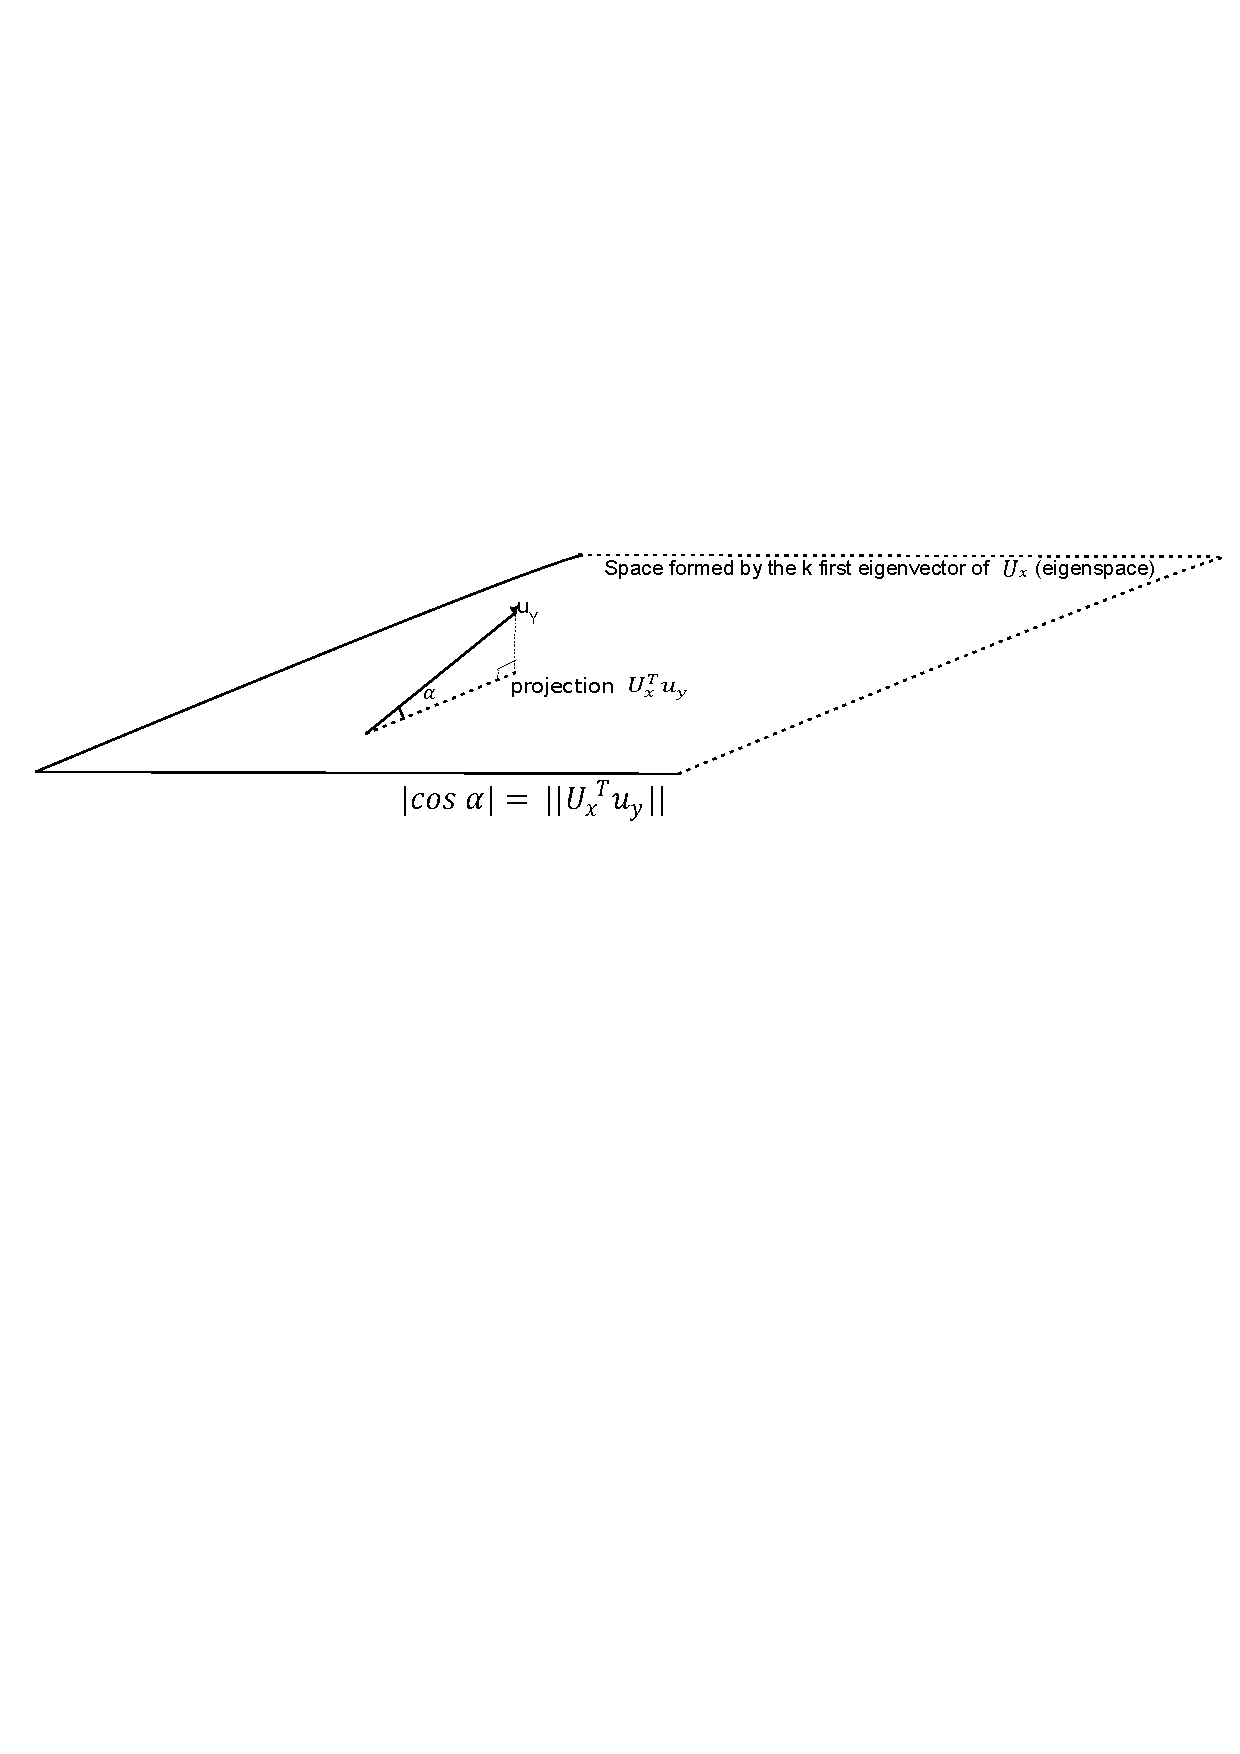
\includegraphics[scale=0.70]{images/loco2}
\caption{Geometric representation of loco similarity.}
\label{geoLoco}
\end{figure}


Intuitively, two time series X and Y will be considered as close when the angle
$\alpha$ formed by the space carrying the information of the time series X and
the vector carrying the information the time series Y is zero. In other words X
and Y will be close when the value of the $cos(\alpha)$ will be 1. The only
assumption made for the computation of LoCo similarity is that the mean of time
series data point is zero. This could be easily achieve with z-normalization.
LoCo similarity function has many interesting properties and does not require to:
\begin{itemize}
  \item Know the probability distribution of the uncertainty,
  \item Assume the independence of the random variables or the length of
  u-shapelets.
\end{itemize}

It is therefore interesting for feature selection, but we still need a dissimilarity
function to be able to discover u-shapelet. In the next paragraph, we 
define a dissimilarity function that has the same properties as LoCo and that is
robust to the presence of uncertainty.

\section{Our Approach}
\subsection{Dissimilarity function}

The LoCo similarity function defined on two multivariate time series X and Y approximately corresponds  to the absolute value of the cosine of the angle formed by the eigenspaces of X and Y ($|cos(\alpha)|$). A straightforward idea would be to use the $sin(\alpha)$ or $\alpha$-value as a dissimilarity function but this approach does not work so well; the sine and the angle are not discriminant enough for eigenvector comparison for clustering purpose. We thus propose the following dissimilarity measure (Definition. \ref{FOTS}). 


\begin{definition}
\label{FOTS}
(FOTS : Frobenius cOrrelation for uncertain Time series uShapelet discovery) Given two series $X$
and $Y$, their FOTS score is defined by
\begin{eqnarray}
FOTS(X,Y)=\Vert U_{X}-U_{Y}\Vert_{F}
=\sqrt{\stackrel[i=1]{m}{\sum}\stackrel[j=1]{k}{\sum}(U_{X}-U_{Y})_{ij}^{2}}
\end{eqnarray}
where $\Vert\Vert_{F}$ is the Frobenius norm.
\end{definition}
 
 Because the FOTS computation is based on the comparison of the k-first eigenvectors of the autocorrelation
 matrices of the time series, it has the same desirable properties of the LoCo
 similarity function, that is: 
 
 \begin{itemize}
   \item It \textbf{allows to capture complex relationship}
in time series like the key oscillatory (e.g., sinusoidal) as well as aperiodic (e.g.,
increasing or decreasing) trends that are present;
   \item It allows to \textbf{reduce the sensibility to transient changes} in time
   series;
   \item It is appropriate for the \textbf{comparison of short
   timeseries}.
 \end{itemize}

  Moreover, the FOTS dissimilarity function is \textbf{robust to the presence of
  uncertainty} due to the spectral decomposition of the autocorrelation matrices of the time series. The robustness of FOTS to the uncertainty is confirmed by the following theorem:   

\begin{theorem}
\textbf{(Hoffman\-Wielandt)} \cite{Bhatia1993} If $X$ and $X + E$ are $n \times
n$ symmetric matrices, then : 
\begin{eqnarray}
\stackrel[i=1]{n}{\sum}(\lambda_{i}(X+E)-\lambda_{i}(X))^{2}\leq||E||_{F}^{2}.
\end{eqnarray}
where $\lambda_i(X)$ is the ith largest eigenvalue of $X$, and $||E||_{F}^{2}$
is the squared of the Frobenius norm of E.
\end{theorem}

The next section explains how FOTS is integrated in the Scalable Unsupervised Shapelet discovery algorithm.


\subsection{Scalable u-shapelets Algorithm with FOTS score}
In this section we do not define a new SUShapelet algorithm, but we explain how we use SUShapelet algorithm with FOTS score (FOTS-SUSh) to deal with uncertainty.


 Two main criteria make  possible to evaluate the quality of a u-shapelet:
\begin{itemize}
  \item It has to produce two r-balanced groups.
  \item It must build two well separated groups, i.e., groups whose gap is
  maximal.
\end{itemize}

The gap is, therefore, an essential criterion for the selection of u-shapelets candidate. It is subject to uncertainty because its calculation is based on the
Euclidean distance. To remedy this, we propose to use the FOTS score instead of
a simple Euclidean distance when calculating the gap in the Scalable u-shapelet algorithm. Algorithms \ref{algo1} and \ref{algo2} present a more formal definition:    


 \begin{definition}
The sub-sequence FOTS dissimilarity $\boldsymbol{sd_f(S, T)}$ between
a time series T and a sub-sequence S is the minimum of the FOTS
score between the sub-sequence S and all possible
sub-sequences of T of length equal to the length of S.
\end{definition}


\begin{algorithm}[h]
\DontPrintSemicolon
\KwIn{u-shapeletCandidate : s,\\ time series dataset : D}
\KwOut{Distance between the u-shapelet Candidate and all the time series of the
dataset}
\SetKwBlock{Begin}{function}{end function}

\Begin($\text{ComputeOrderline} {(} s, \, D{)}$)
{
  $dis \leftarrow \{\}$\;
  $s \leftarrow zNorm(s)$\;
  \ForAll{$i \in \left\lbrace  1, 2, \ldots, |D|\right\rbrace$}
  {
    $ts \leftarrow D(i,:)$\;
    $dis(i) \leftarrow sd_f(s,ts)$\;    
  }  
  \Return{$\nicefrac{dis}{|s|}$}

}
\caption{ComputeOrderline}
\label{algo1}
\end{algorithm}



\begin{algorithm}[h]
\DontPrintSemicolon
\KwIn{u-shapeletCandidate : s,\\ 
timeseries dataset : D, \\
lb, ub : lower/upper bound of reasonable number of time series in cluster}
\KwOut{gap : gap score}
\SetKwBlock{Begin}{function}{end function}

\Begin($\text{ComputeGap} {(} s, \, D, \, lb, \, ub{)}$)
{
  $dis \leftarrow ComputeOrderline(s,D)$\;
  $gap \leftarrow 0$\;
  
     \For{$i \leftarrow lb \, \boldsymbol{to} \, ub$}
    {
        $D_A \leftarrow dis \leq dis(i)$,
        $D_B \leftarrow dis > dis(i)$
        
      \uIf{$lb \leq |D_A| \leq ub$}
      {
       $m_A \leftarrow mean(D_A) $,
       $ m_B \leftarrow mean(D_B)$\;
       
       $s_A \leftarrow std(D_A)$,
       $s_B \leftarrow std(D_B)$\;
       
       $currGap \leftarrow m_B - s_B - (m_A + s_A)$
       
       \uIf{$currGap > gap$}
       {
       	$gap \leftarrow currGap$
       } 
      }
    }  
  \Return{$gap$}

}
\caption{ComputeGap}
\label{algo2}
\end{algorithm}

\section{Experimental Evaluation}

\subsection{Clustering with u-shapelets}
The algorithm iteratively splits the data with each discovered u-shapelet: each u-shapelet splits the dataset into two groups $D_A$ and $D_B$. The time series that belong to $D_A$ are considered as members of the cluster form by the u-shapelet and are then removed from the dataset. A new u-shapelet search continues with the rest of the data until there is no more time series in the dataset or until the algorithm is no more able to find u-shapelet. As a stopping
criterion for the number of u-shapelets extracted, the decline of the u-shapelet gap score is
examined: the algorithm stops when the gap score of the newly-found u-shapelet
becomes less than half of the gap score of the first discovered u- shapelet. This approach is a direct implementation of the u-shapelet definition

\paragraph{Choosing the length $N$ of a uShapelet : }
The choice of the length of u-shapelet is directed by the knowledge of the
domain to which the time series belongs. As part of these experiments, we tested all  numbers between 4 and half the length of the time series. We consider as length of u-shapelet the one allowing to better cluster the time series.

\paragraph{Choosing the length $w$ of the windows : }
The use of overlapping windows for calculating the autocorrelation matrix makes
it possible to capture the oscillations present in the time series. During these experiments, we consider that the size of the window is equal to half the length of the u-shapelet.
  
\paragraph{Choosing  the number $k$ of eigenvectors: }
A practical choice is to fix $k$ to a small value; we use $k = 4$ throughout all
experiments. Indeed, key aperiodic trends are captured by one eigenvector,
whereas key oscillatory trends manifest themselves in a pair of eigenvectors.  

\subsection{Evaluation Metric}
Different measures for time series clustering quality have been proposed, including Jaccard Score, Rand Index, Folkes and Mallow index, etc. However, because in our case we have ground truth class labels for the datasets, we can use this external information to evaluate the true clustering quality by using Rand Index. Moreover, Rand Index appears to be the most commonly used clustering quality measure \cite{zakaria2012clustering, ulanova2015scalable, zhang2016unsupervised}, and many of the other measures can be seen as minor variants of it\cite{halkidi2001clustering}.
To appreciate the quality of the u-shapelets found, we use them for a clustering task. The quality of clustering is evaluated from the Rand Index \cite{rand1971objective} which is calculated as follows:

Let Lc be the cluster labels returned by a clustering algorithm and Lt be the
set of ground truth class labels. Let A be the number of time series that are
placed in the same cluster in Lc and Lt, B be the number of time series in
different clusters in Lc and Lt, C be the number of time series in the same
cluster in Lc but not in Lt and D be the number of time series in different
clusters in Lc but in same cluster in Lt. The Rand Index is equals to : 

\begin{eqnarray}
Rand\,Index = (A+B)/(A+B+C+D)
\end{eqnarray}    

\subsection{Comparison with u-shapelet}
All measurements performed by a mechanical system have uncertainty. Indeed, the uncertainty principle is partly a statement about the limitations of mechanical systems ability to perform measurements on a system without disturbing it \cite{folland1997uncertainty}. So, similarly to \cite{dallachiesa}, we tested our method on 17 real world datasets coming from UCR archive \cite{UCRArchive} representing a wide range of application domains. The training and testing sets have been joined to obtained bigger datasets. Table \ref{datasets} present detailed information about tested datasets.




\begin{table}[ht]
\centering
\small
\begin{tabular}{lcccl}
\textbf{Data-set}   & \textbf{Size of  } & \textbf{Length} & \textbf{No. of  } & \textbf{Type} \\
\textbf{ }   & \textbf{  dataset} & \textbf{ } & \textbf{  Classes} & \textbf{ } \\
50words            & 905                      & 270             & 50                      & IMAGE         \\
Adiac              & 781                      & 176             & 37                      & IMAGE         \\
Beef               & 60                       & 470             & 5                       & SPECTRO       \\
Car                & 120                      & 577             & 4                       & SENSOR        \\
CBF                & 930                      & 128             & 3                       & SIMULATED     \\
Coffee             & 56                       & 286             & 2                       & SPECTRO       \\
ECG200             & 200                      & 96              & 2                       & ECG           \\
FaceFour           & 112                      & 350             & 4                       & IMAGE         \\
FISH               & 350                      & 463             & 7                       & IMAGE         \\
Gun\_Point         & 200                      & 150             & 2                       & MOTION        \\
Lighting2          & 121                      & 637             & 2                       & SENSOR        \\
Lighting7          & 143                      & 319             & 7                       & SENSOR        \\
OliveOil           & 60                       & 570             & 4                       & SPECTRO       \\
OSULeaf            & 442                      & 427             & 6                       & IMAGE         \\
SwedishLeaf        & 1125                     & 128             & 15                      & IMAGE         \\
synthetic\_control & 600                      & 60              & 6                       & SIMULATED     \\
FaceAll            & 2250                     & 131             & 14                      & IMAGE        
\end{tabular}
\caption{Datasets}
\label{datasets}
\end{table}

Table \ref{ri} presents the comparison of the two algorithms.

\begin{table}[ht]
\centering
\begin{tabular}{lcc}
\textbf{Datasets}  & \textbf{RI\_SUSh} & \textbf{RI\_FOTS} \\
50words            & 0.811             & \textbf{0.877}    \\
Adiac              & 0.796             & \textbf{0.905}    \\
Beef               & 0.897             & \textbf{0.910}    \\
Car                & 0.708             & \textbf{0.723}    \\
CBF                & 0.578             & \textbf{0.909}    \\
Coffee             & 0.782             & \textbf{0.896}    \\
ECG200             & 0.717             & \textbf{0.866}    \\
FaceFour           & 0.859             & \textbf{0.910}    \\
FISH               & 0.775             & \textbf{0.899}    \\
Gun\_Point         & 0.710             & \textbf{0.894}    \\
Lighting2          & 0.794             & \textbf{0.911}    \\
Lighting7          & 0.757             & \textbf{0.910}    \\
OliveOil           & 0.714             & \textbf{0.910}    \\
OSULeaf            & 0.847             & \textbf{0.905}    \\
SwedishLeaf        & 0.305             & \textbf{0.909}    \\
synthetic\_control & 0.723             & \textbf{0.899}    \\
FaceAll            & 0.907             & \textbf{0.908}   
\end{tabular}
\caption{Comparison of the Rand Index of SUSH (RI\_SUSh) and FOTS-SUSh (RI\_FOTS). The best Rand Index is in bold}
\label{ri}
\end{table}

\subsection{Comparison with k-Shape and USLM}

k-Shape and USLM are two u-shapelets  based clustering algorithms for time series presented in \cite{zhang2016unsupervised}. In this section, we compare the Rand Index obtained by FOTS-UShapelet and the one obtained by k-Shape and USLM on 5 datasets(Table \ref{comparison_rand_index}). The results of k-Shape and USLM was previously reported in \cite{zhang2016unsupervised}. This comparison shows that in general, FOTS-UShapelet perform better than k-Shape and USLM.

\begin{table}[h]
\centering
\caption{Comparison between k-Shape, USLM and FOTS-UShapelet}
\label{comparison_rand_index}
\begin{tabular}{llll}
\textbf{\begin{tabular}[c]{@{}l@{}}Rand\\   Index\end{tabular}} & \textbf{k-Shape} & \textbf{USLM} & \textbf{FOTS-UShapelet} \\
CBF                                                             & 0.74             & \textbf{1}    & 0.909                   \\
ECG200                                                          & 0.70             & 0.76          & \textbf{0.866}          \\
Fac.F.                                                          & 0.64             & 0.79          & \textbf{0.910}          \\
Lig2                                                            & 0.65             & 0.80          & \textbf{0.911}          \\
Lig.7                                                           & 0.74             & 0.79          & \textbf{0.910}          \\
OSU L.                                                         & 0.66             & 0.82          & \textbf{0.905}         
\end{tabular}
\end{table}

				
\subsection{Discussion}

The use of the FOTS score associated with the SUShapelet algorithm makes it
possible to discover different u-shapelets than those found by the Euclidean
distance. The FOTS-SUSh improves the results of time series clustering because the FOTS score takes into account the intrinsic properties of the time series when searching for u-shapelets and is robust to the presence of uncertainty. This improvement is particularly significant when the FOTS score is used for the clustering of time series containing several small oscillations. Indeed, these oscillations are not captured by the Euclidean distance but are by the FOTS score whose calculation is based on the autocorrelation matrix. This observation is illustrated by the result obtained on  SwedishLeaf dataset.

\subsubsection{Time complexity analysis} ED can be computed in $\mathcal{O}(n)$ and  FOTS score is computed in $\mathcal{O}(n^\omega),\:2\leq\omega\leq3$ due to the time complexity of the eigenvector decompositions \cite{pan1999complexity}. The computation of FOTS score is then more expensive than that of ED (Fig. \ref{temps_ED_FOTS}). However, its use remains relevant for u-shapelet research as they are often small.


 \begin{figure}[h]
  \centering
   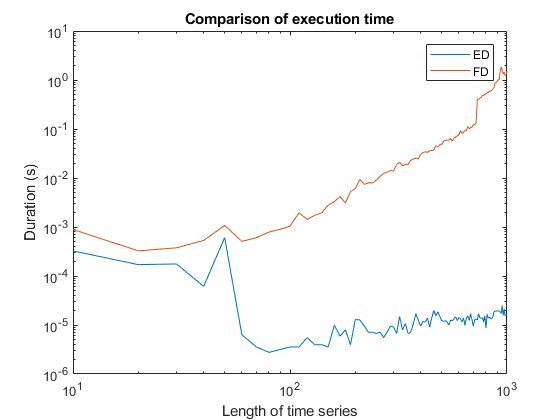
\includegraphics[scale=0.5]{images/temps_ED_FOTS}
    \caption{Comparison between the execution time of the Euclidean distance and that of the FOTS score as a function of the length of the time series}
  \label{temps_ED_FOTS}
  \end{figure}

\section{Conclusion and Future Work}
The purpose of this work was to discover u-shapelets on uncertain time series. To answer this question, we have proposed a dissimilarity score (FOTS) adapted to the comparison of short time series, whose computation is based on the comparison of the eigenvector of the autocorrelation matrices of the time series. This score is robust to the presence of uncertainty, it is not very sensitive to transient changes, and it allows capturing complex relationships between time series such as oscillations and trends. The FOTS score was used with the Scalable Unsupervised Shapelet Discovery algorithm for clustering 17 literature datasets and showed an improvement in the quality of clustering evaluated using the Rand Index.  By combining the benefits of the u-shapelets algorithm, which reduces the adverse effects of uncertainty, and the benefits of the FOTS score, which is robust to the presence of uncertainty, this work is defining a framework for clustering uncertain time series. As a perspective to this work, we plan to use the FOTS score for fuzzy clustering of uncertain time series.
